
關於C++內存管理的主題可以單獨成書。關於STL分配器的問題,的論文很多。本章中,將重點討論幾個影響性能的問題。有些有簡單的解決方案。其他的,我們將描述問題,並概述可能的解決方法。 

性能方面可能會遇到兩種與內存相關的問題。第一個問題是使用太多內存:程序要麼耗盡內存,要麼沒有滿足內存使用要求。第二個問題發生在程序受到內存限制時,性能受到內存訪問速度的限制。在這樣的情況下,程序的運行時間與使用的多少內存直接相關,減少內存使用會使程序運行得更快。 

本節中介紹的示例適用於處理內存限制程序或頻繁和/或大量分配內存的程序。我們從內存分配本身對性能的影響開始。

\subsubsubsection{9.4.1\hspace{0.2cm}不必要的內存分配}

與內存使用相關的性能問題之一是\textit{不必要的內存分配}。下面是一個常見的問題,用類似C++的偽代碼來描述:

\begin{lstlisting}[style=styleCXX]
for ( … many iterations … ) {
	T* buffer = allocate(… size …);
	do_work(buffer); // Computations use memory
	deallocate(buffer);
}
\end{lstlisting}

良好的程序會使用RAII類來管理回收內存,但是為了清晰明瞭,希望使顯式分配和回收。分配通常隱藏在管理自己內存的對象中,比如STL容器。這樣會將大部分時間花在內存分配和回收函數(如\texttt{malloc()}和\texttt{free()})上。 

可以在基準測試中看到它對性能的影響:

\hspace*{\fill} \\ %插入空行
\noindent
\textbf{04\_buffer.C}
\begin{lstlisting}[style=styleCXX]
void BM_make_str_new(benchmark::State & state) {
	const size_t NMax = state.range(0);
	for (auto _: state) {
		const size_t N = (random_number() % NMax) + 1;
		char * buf = new char[N];
		memset(buf, 0xab, N);
		delete[] buf;
	}
	state.SetItemsProcessed(state.iterations());
}
\end{lstlisting}

這裡是通過初始化一個字符串來表示的,\texttt{random\_number()}返回隨機整數值(可能只是\texttt{rand()},但是若預先計算和存儲隨機數,以避免對隨機數生成器進行基準測試,那麼基準測試會更簡潔)。可能還需要哄騙編譯器不要優化掉結果,若\texttt{benchmark::DoNotOptimize()}不能滿足要求,可能需要插入一個\texttt{print}語句,但條件永遠不會發生(但編譯器並不知道),比如\texttt{rand() < 0}。

從基準中得到的數據沒什麼意義,需要與其他東西進行比較才可以。我們的例子中,基線很容易確定,可以做相同的工作,但不進行分配。這可以通過將分配和回收移出循環來實現(已知最大內存大小):

\hspace*{\fill} \\ %插入空行
\noindent
\textbf{04\_buffer.C}
\begin{lstlisting}[style=styleCXX]
char * buf = new char[NMax];
for (auto _: state) {
	…}
delete[] buf;
\end{lstlisting}

基準測試中,觀察到的性能差異在很大程度上取決於操作系統和系統庫,但很可能會看到這樣的情況(使用的是隨機大小為1KB的字符串):

%\hspace*{\fill} \\ %插入空行
\begin{center}
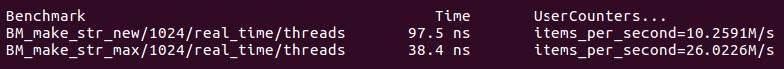
\includegraphics[width=0.9\textwidth]{content/3/chapter9/images/5.jpg}\\
圖9.5 - 分配-回收模式對性能的影響
\end{center}

與內存分配模式複雜得多的大型程序相比,微基準測試中的內存分配通常更高效,因此頻繁的分配和回收在實際中的影響可能更大。即使在我們的微基準測試中,每次分配內存的實現運行速度只有一次分配最大可能內存量的版本的40\%。 

如果在計算過程中所需要的最大內存是已知的,那麼預先分配內存並從一個迭代到下一個迭代進行重用,就是一個簡單的解決方案。這個解決方案也適用於許多容器,對於\texttt{vector}或\texttt{deque}容器來說,利用調整容器大小不會縮小其容量的事實,可以在迭代開始之前預留內存。

如果事先不知道最大內存大小,解決方案就會複雜一些。這種情況可以使用僅增長的緩衝區來處理。下面是一個簡單的緩衝區,只能增長:

\hspace*{\fill} \\ %插入空行
\noindent
\textbf{04\_buffer.C}
\begin{lstlisting}[style=styleCXX]
class Buffer {
	size_t size_;
	  std::unique_ptr<char[]> buf_;
	public:
	explicit Buffer(size_t N) : size_(N), buf_(
	new char[N]) {}
	void resize(size_t N) { 
		if (N <= size_) return;
		char* new_buf = new char[N];
		memcpy(new_buf, get(), size_);
		buf_.reset(new_buf);
		size_ = N;
	}
	char* get() { return &buf_[0]; }
};
\end{lstlisting}

同樣,這段代碼對於演示和探索都非常有用。實際中,可能會使用STL容器或自己的庫類,但它們都應該具有增加內存容量的能力。可以通過簡單地修改基準測試,來比較這個只增長的緩衝區和固定大小的預分配緩衝區的性能:

\hspace*{\fill} \\ %插入空行
\noindent
\textbf{04\_buffer.C}
\begin{lstlisting}[style=styleCXX]
void BM_make_str_buf(benchmark::State& state) {
	const size_t NMax = state.range(0);
	Buffer buf(1);
	for (auto _ : state) {
		const size_t N = (random_number() % NMax) + 1;     
		buf.resize(N);
		memset(buf.get(), 0xab, N);
	}
	state.SetItemsProcessed(state.iterations());
}
\end{lstlisting}

現實中,使用更智能的內存增長策略可能會得到更好的結果(比請求的內存增長稍微多一些,所以不必經常增加內存——大多數STL容器都採用這種策略)。但在我們的演示中,想讓事情儘可能的簡單。在同一臺機器上,基準測試的結果如下:

%\hspace*{\fill} \\ %插入空行
\begin{center}
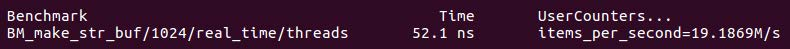
\includegraphics[width=0.9\textwidth]{content/3/chapter9/images/6.jpg}\\
圖9.6 - 只增長緩衝區的性能(與圖9.5相比)
\end{center}

只增長的緩衝區比固定大小的緩衝區慢,但比每次分配和回收內存都會快很多。同樣,更好的增長政策將使這個緩衝更快,接近固定大小的速度。 

多線程程序中,良好的內存管理更為重要,因為對系統內存分配器的調用不能很好地擴展,並且可能涉及全局鎖。同一臺機器上使用8個線程運行基準測試會產生以下結果:

%\hspace*{\fill} \\ %插入空行
\begin{center}
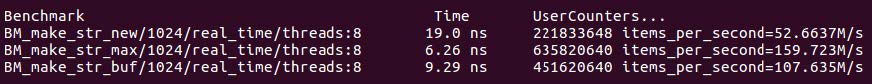
\includegraphics[width=0.9\textwidth]{content/3/chapter9/images/7.jpg}\\
圖9.7 - 多線程程序中分配-回收模式對性能的影響
\end{center}

這裡,頻繁分配的代價更大(只增長緩衝區也展示了分配剩餘內存的成本,從而從好的增長策略中受益)。 

儘可能少地與操作系統交互。如果有一個循環需要在每次迭代中分配和釋放內存,那麼在循環之前分配。如果分配的大小相同,或者預先知道最大分配大小,則預分配一個這個大小的內存,並保持它(當然,如果使用幾個緩衝區或容器,不應該將它們硬塞到一個分配中,而是應該為每個區域進行預分配)。如果不知道最大內存大小,則使用可以增長的數據結構,但在工作完成之前不要縮減或釋放內存。 

避免與操作系統交互的建議在多線程程序中尤為重要,現在我們將對併發程序中的內存使用做一些討論。

\subsubsubsection{9.4.2\hspace{0.2cm}併發程序中的內存管理}

操作系統提供的內存分配器是一種平衡多種需求的解決方案。在給定的機器上,只有一個操作系統,但有許多不同的程序,它們有自己獨特的需求和內存使用模式,開發人員非常努力地讓它在合理的使用方式中不會失敗。另一方面,它也很少是最佳解決方案。通常,這已經足夠好了,特別是如果需要頻繁的申請內存。

在併發程序中,內存分配變得更加低效。主要原因是,內存分配器都必須維護相當複雜的內部數據結構,以跟蹤分配和釋放內存。在高性能分配器中,內存會細分為多個方面,以便將類似大小的分配組合在一起。這就是以複雜性為代價,提高了性能。如果多個線程同時分配和釋放內存,那麼內部數據的管理必須由鎖來保護。這是一個全局鎖,用於整個程序,如果經常調用分配器,它會限制整個程序的擴展性。

這個問題最常見的解決方案是使用帶有線程局部緩存的分配器,比如流行的\texttt{malloc()}替換庫TCMalloc。這些分配器為每個線程預留了一定數量的內存,當一個線程需要分配內存時,首先從線程本地內存域中獲取。這並不需要鎖,因為只有一個線程與該域交互。只有當域為空時,分配器才必須從所有線程共享的內存中獲取鎖並進行分配。當一個線程釋放內存時,釋放的內存會添加到線程特定域中,同樣不需要任何鎖。

線程本地緩存也不是沒有問題。

首先,它們傾向於使用更多的內存。如果線程釋放了大量內存,而另一個線程分配了大量內存,那麼最近釋放的內存對另一個線程來說是不可用的(對於釋放它的線程來說內存是本地的)。因此,當未使用的內存可供其他線程使用時,會分配更多的內存。為了限制這種內存浪費,分配器通常不允許每個線程的空間增長超過某個預定義的限制。達到限制時,線程本地內存將返回到所有線程共享的內存域中(這個操作需要一個鎖)。

其次,如果每個分配都由一個線程擁有,這些分配器可以工作得很好,相同的線程可以在每個地址分配和釋放內存。如果一個線程分配了一些內存,另一個線程必須釋放,因為內存必須從一個線程的局部域,轉移到另一個線程的局部域(或共享域),所以這種跨線程釋放很困難。基準測試表明,使用標準分配器(如\texttt{malloc()}或TCMalloc)的跨線程回收的性能,至少比線程分別擁有本地內存的性能差一個數量級。對於使用線程本地緩存的分配器來說,這可能都是正確的,因此應該儘可能避免線程之間的內存交互。

現在,我們討論的是將內存從一個線程傳輸到另一個線程,目的是回收內存。那麼簡單地使用由另一個線程分配的內存呢?這種內存訪問的性能在很大程度上取決於硬件能力。對於CPU較少的簡單系統,這可能不是問題。但是較大的系統有多個內存庫,並且CPU和內存之間的連接是不對稱的。每個內存庫更接近一個CPU,這就是所謂的\textbf{非均勻內存訪問(NUMA)}。NUMA對性能的影響差別很大,\textit{從無關緊要到快了一倍}。有一些方法可以優化NUMA內存系統的性能,並使程序內存管理對NUMA敏感。但請注意,您可能會針對特定的機器調優性能,但關於NUMA系統的一般性性能資料,可以幾乎沒有。

我們現在回到更有效地使用內存的問題,因為它對併發程序和串行程序的性能都有幫助。

\subsubsubsection{9.4.3\hspace{0.2cm}避免內存碎片}

困擾許多程序的問題是與內存分配系統的低效交互。假設程序需要分配1KB的內存。這個內存塊是從一些更大的內存空間中取出來的,標記為由分配器使用,並將地址返回給調用者。接下來會分配更多的內存,所以1KB塊之後的內存現在也使用了。然後程序返回第一個分配,並立即請求2KB的內存。這時有一個1KB的空閒塊,但它不夠大,不能滿足新的請求。其他地方可能還有另一個1KB的塊,但只要這兩個塊不是緊挨著的,則對於2KB的分配申請就沒什麼意義:

%\hspace*{\fill} \\ %插入空行
\begin{center}
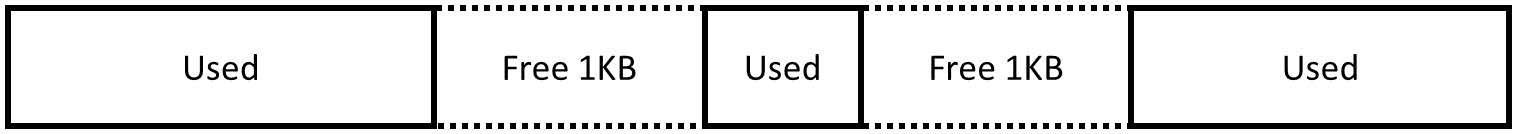
\includegraphics[width=0.9\textwidth]{content/3/chapter9/images/8.jpg}\\
圖9.8 - 內存碎片:存在2KB的空閒內存,但對於單個2KB的分配並沒啥用
\end{center}

這種情況稱為\textbf{內存碎片}:系統有程序返回的空閒內存,但必須使用新的內存來服務於下一次分配,因為程序釋放的內存分割成小塊。在極端的情況下,這種碎片可能會導致程序在系統的總內存容量耗盡之前就“耗盡內存”(作者所見過的最糟糕的情況是,一個程序在只分配了總可用內存的1/6後就“耗盡”了內存)。有些內存分配器比標準的\texttt{malloc()}更能抗碎片,但是對於快速移動內存的程序,可能需要更極端的措施。

一種解決方式為塊分配器,所有內存都以固定大小的塊(比如64KB)分配。不能從操作系統一次分配一個這樣大小的塊,而是分配較大的內存塊(例如,8MB),並將它們細分為較小的塊(在我們的示例中為64KB)。處理這些請求的內存分配器是程序中的主分配器,直接與\texttt{malloc()}交互。因為只分配一個大小的塊,所以非常簡單,這樣我們就可以專注於最有效的實現(併發程序的線程本地緩存,實時系統的低延遲等)。當然,誰都不想在代碼中處理這些64KB的塊(其實這是二級分配器的工作),如圖9.9所示:

%\hspace*{\fill} \\ %插入空行
\begin{center}
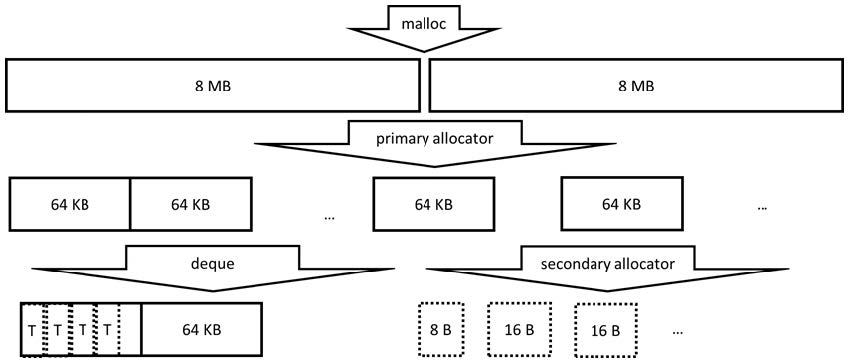
\includegraphics[width=0.9\textwidth]{content/3/chapter9/images/9.jpg}\\
圖9.9 - 固定大小的塊分配
\end{center}

可以使用分配器將64KB的塊進一步細分為更小的塊。統一分配器(只分配一個大小的分配器)非常高效,為單個64位整數分配內存,就可以這樣做,而不需要任何內存開銷(相比之下,\texttt{malloc()}每次分配通常需要至少16個字節的開銷)。還可以使用容器以64KB塊分配內存,並使用它來存儲元素。這裡不會使用\texttt{vector},因為它需要一個大型的、連續的分配。這裡需要的容器是\texttt{deque},它在固定大小的塊中分配內存。當然,也可以使用節點容器。如果STL分配器接口足以滿足需求,可以使用STL容器,要不就需要編寫自己的容器庫了。

固定大小的塊分配的優點是不會受到碎片化的影響,\texttt{malloc()}的所有分配都是相同的大小,主分配程序的所有分配也是一樣的。一個內存塊返回給分配器時,都可以重用以滿足下一個內存請求。參考下圖:

%\hspace*{\fill} \\ %插入空行
\begin{center}
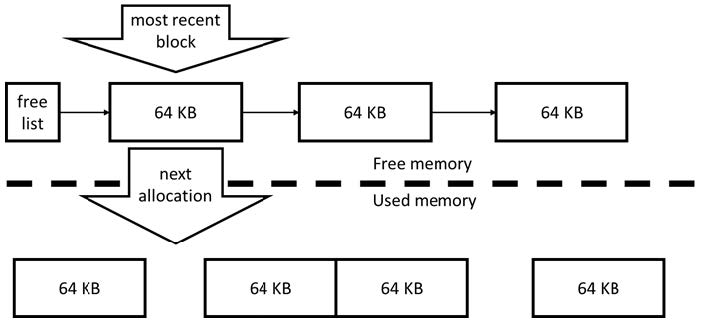
\includegraphics[width=0.9\textwidth]{content/3/chapter9/images/10.jpg}\\
圖9.10 - 固定大小分配器中的內存重用
\end{center}

這種先進先出的屬性也是一個優勢。最後的64KB內存塊很可能來自最近使用的內存,並且在緩存中仍然是\textit{熱的}。重用這個塊可以立即改善內存引用的局部性,因此可以更有效地使用緩存。分配調度器會返回塊作為一個簡單的空閒鏈表(圖9.10)。可以為每個線程維護這些空閒鏈表,以避免鎖的使用,可能需要定期重新平衡,以避免線程積累了過多的空閒塊,而另一個線程正在分配新內存的情況。

當然,將64KB塊細分成更小大小的分配器時,仍然容易受到碎片的影響,除非也是統一(固定大小)的分配器。然而,如果必須處理較小的內存(一個塊)和少量不同大小的內存,那麼編寫一個可以自動進行碎片整理分配器會更容易。 

使用塊內存分配的決定很可能會影響整個程序,例如:分配大量的小數據結構,使每個數據結構使用64KB塊的一小部分,這將降低內存的性價比。另一方面,如果數據結構本身是一組較小的數據結構(容器)的集合,可以將許多較小對象打包到一個塊中,那麼這種數據結構就更容易處理。甚至可以編寫壓縮容器來壓縮每個塊,以便長期保存數據,然後進行解壓縮以便訪問。 

區塊大小本身也不是一成不變的。一些應用程序使用更小的塊會更有效率,如果塊部分未使用,內存浪費更少。其他線程可以減少大內存塊分配的次數,從而在性能上獲益。

關於特定於應用程序的分配器的文獻非常豐富,例如:slab分配器是剛才看到的塊分配器的泛化版本,可以有效地管理多個內存分配。還有許多其他自定義的內存分配器,其中大多數都可以在C++中使用。特定應用程序的分配器通常會帶來顯著的性能改進,但代價通常是嚴重限制了開發者實現數據結構的自由。

下一個導致效率低下的常見原因更為微妙,也更難處理。





















